\documentclass[titlepage]{article}%
%Options -- Point size:  10pt (default), 11pt, 12pt
%        -- Paper size:  letterpaper (default), a4paper, a5paper, b5paper
%                        legalpaper, executivepaper
%        -- Orientation  (portrait is the default)
%                        landscape
%        -- Print size:  oneside (default), twoside
%        -- Quality      final(default), draft
%        -- Title page   notitlepage, titlepage(default)
%        -- Columns      onecolumn(default), twocolumn
%        -- Equation numbering (equation numbers on the right is the default)
%                        leqno
%        -- Displayed equations (centered is the default)
%                        fleqn (equations start at the same distance from the right side)
%        -- Open bibliography style (closed is the default)
%                        openbib
% For instance the command
%           \documentclass[a4paper,12pt,leqno]{article}
% ensures that the paper size is a4, the fonts are typeset at the size 12p
% and the equation numbers are on the left side
%
\usepackage{amsmath}%
\usepackage{amsfonts}%
\usepackage{amssymb}%
\usepackage{graphicx}

\newcommand{\HRule}{\rule{\linewidth}{0.5mm}}

\begin{document}
\begin{titlepage}
 
\begin{center}
 
 
% Upper part of the page
\HRule \\[3cm]


\includegraphics[scale=0.45]{diagrams/header_logo}\\[1.5cm]
 
\textsc{\LARGE Developer's Guide}\\[3cm]
 
\HRule 
 
\vfill
 
% Bottom of the page
A.Davoust \\
\today
 
\end{center}
 
\end{titlepage}

\tableofcontents
\newpage
%---------------------------------------------------------------

\section{Introduction}
Welcome to Universal Peer-to-Peer (U-P2P) Developer's Guide!

This guide is targeted at software developers who are interested in the implementation of U-P2P and its inner workings. 

U-P2P is a file-sharing client working as an overlay over the Gnutella network\footnote{earlier versions worked with multiple networks, such as JXTA and Napster-type networks, but the current version only includes the Gnutella Network Adapter. U-P2P could easily be customized for other networks.}.

The specificity of U-P2P as compared to traditional file-sharing systems is that files shared in U-P2P come with XML metadata, and can be of many different types. We have built a number of additional features relying on the XML-centered file-sharing infrastructure of U-P2P, including links between documents, and possibilities for any user to publish new types of documents with their own metadata schemas.

Section \ref{sec:concept} gives an overview of U-P2P, its general concept, features, and high-level design.

U-P2P is implemented in Java, and runs as a Web Application under Apache Tomcat\footnote{this is the main way of running U-P2P, although some parts can be run as a standalone java application, see section \ref{standalone}}, and thus leverages the powerful rendering tools offered by XML / XSLT and a web browser.

As a file-sharing client, U-P2P comprises four three functional modules : 
\begin{itemize}
\item a user interface, built using Java Servlets and Java Server Pages (JSP), and making use of the Tomcat Servlet Engine
\item an XML database, built using an early version of the eXist\footnote{http://exist-db.org/} XML Database.
\item a Network Adapter, built over the JTella library to use the Gnutella protocol.
\end{itemize}
These functional modules are coordinated through a tuple space. 

Section \ref{sec:functionalspec} provides a functional specification of U-P2P as a whole, and of each functional module.

Sections \ref{sec:UIDesign}, \ref{sec:RepositoryDesign}, \ref{sec:NetworkAdapterDesign}, and \ref{sec:TSDesign} detail the object-oriented design of the three functional modules, and of the tuple space framework.

Section \ref{sec:ExtensionsDesign} covers extensions such as the U-P2P console mode and RDF Adapter (which is under construction)

Finally the last section of this document, section \ref{sec:ConfigTesting} will address practical issues such as configuration, testing, etc.

%==================================================================================================================
\section{Overview of U-P2P}
\label{sec:concept}
\subsection{General Concept}
\paragraph{What is U-P2P?}
In a few words, U-P2P is a client for sharing files and their XML meta-data in a P2P network. XML documents are stored in XML databases on the users' computers, and P2P connections allow the peers to share documents with one another. This section gives an overview of the main concepts we use in U-P2P.

U-P2P is a research project based at Carleton University's NMAI lab.

\paragraph{What U-P2P is not}
A client for downloading regular music and video files from traditional P2P networks, a bittorrent client. 

\paragraph{Documents}
In U-P2P, files such as text documents or music files are bundled together with their metadata, as XML documents with ``attachments'' similar to email attachments. XML documents may also describe non-electronic objects (e.g stamps or molecules), which would then have an independent existence --- and then only the XML metadata is shared in U-P2P.

In this guide we will use alternatively the terms \emph{Document} and \emph{Resource}.

\paragraph{Communities}
Based on the idea that groups of users sharing the same type of files can be considered \emph{communities}, we define a community by the common pattern of the meta-data (schema) describing the files. For example, a schema for describing mp3-encoded music files could be the list of attributes [artist, title, album, year, genre, bitrate]. Based on this schema we define a community of users interested in sharing mp3 music files, who use this common schema.

In the same way we can define, for example, a community of users interested in sharing bibtex entries describing science papers, based on a schema of bibliographic information, or a community of users sharing XML-encoded legal proceedings.

As a community is defined by the type of documents shared between its members, we will shortcut and use the term ``community" to designate the collection of documents itself.

\paragraph{Community Definition Documents}
The main interest of the UP2P data model is that a community can be described by a structured XML document: this document lists the community name, a short description, and includes the metadata schema; such documents can be considered resources of a greater ``community of communities" (which we call the Root Community), and in turn shared on the network. This way, in addition to searching for music files or legal proceedings, one may search the Root Community for new communities, download the community documents and start sharing documents within this community. This ``meta'' level is what makes U-P2P unique and allows users to participate in several communities, and to generate new communities.

\subsection{Features} %--------------------------------------------------------------
\paragraph{Basic File-Sharing Use Cases}
UP2P is primarily a file-sharing application, and its main Use Cases are those of any File-Sharing client, such as LimeWire, Emule, etc.. The main difference is that the documents shared within UP2P, as described above, are typed (i.e. they have a particular \emph{type}) by communities.
Within a given community, a user may :
\begin{itemize}
\item View the community, i.e. list the documents of this community stored in his local database; 
\item View a locally stored document, using a community-specific rendering;
\item Search for documents, using conditions on the document attributes as search criteria, and view the results from the UP2P network; 
\item Download a resource from another peer; 
\item Publish a resource; i.e. create a document following the community-specific template, and store it in the local database, also making it available to other peers;
\item Delete a document from the local database (any copies elsewhere in the network are not affected).
\end{itemize}

\paragraph{Links and Complex Queries}
Another important feature of U-P2P is the possibility of creating links between documents. Any document shared in the network --- in any community --- can be referenced by a unique URI. U-P2P provides a dereferencing mechanism to follow such links. This allows navigation between documents shared in the P2P network, similar to navigation between web pages following traditional HTTP links. However, as documents may be found anywhere in the network, retrieving a document implies first a search over the appropriate community; this is done automatically.

Finally, the collection of interlinked documents can be searched by a specialized query interface. The interlinked documents can be seen as a graph, where each document is a node, and a link to another document is an edge directed towards this other document, and labeled with the attribute where the link is found. In other words, some document A has a number of attributes, following the community schema; and the value of a particular attribute \emph{foobar} may be the URI of another document B; we then have a graph with two nodes A and B, and an edge from A to B labeled \emph{foobar}.

This linking mechanism adds two UP2P specific Use Cases to the previous list:
\begin{itemize}
\item Follow a link : from a document containing a link, the user may navigate to the linked document, directly if it is stored locally, or via an automatic search, if the document is elsewhere in the network;
\item Complex Query: as the collection of documents in the UP2P network can be seen as a graph, \emph{graph queries} can be made on this graph. UP2P includes a graphic interface to form such queries. The specifics of these graph queries are described in section \ref{section:graphqueries}.
\end{itemize}

\paragraph{Console mode}
U-P2P can also be run as a standalone java application, in order to experiment with more technical aspects (e.g. the inner workings of the tuple space), and debug more efficiently.

In this mode, U-P2P offers a simple swing GUI, with a view of the tuples in the tuple space, and a screen to add custom logging while experimenting or debugging. Tuples can be manually injected in the tuple space.

However, in this mode, downloads requested by other peers are not serviced (as these normally run through the Tomcat Server).

For details about the console mode, see section \ref{sec:consolemode}.

\subsection{U-P2P High-Level Design} %------------------------------------------------------------------------------

U-P2P can be seen as a distributed XML database, where different types of documents are stored, and where each peer fully controls a piece of the database. The peer can search the database, and move documents to and from its own piece of the database.

The overall functionality of U-P2P, i.e. of a U-P2P client, can thus be broken down into three functional modules : the local Repository, which is the XML database, the User Interface, which collects user requests, and the Network, which forwards requests to other peers. The principle of our design is that the functional components of U-P2P should be completely decoupled; the repository and the network adapter should be implemented in modules providing atomic ``services" that can be invoked asynchronously through a central coordination component.

We have chosen to base our architecture on a Tuple Space\footnote{For more details on what exactly a Tuple Space is, and how it works, read section\ref{section:tuplespace}}, which constitutes this central coordination component. Agents acting as proxies for the different modules output tuples to the Tuple Space, and have templates which they attempt to match to tuples found in the Tuple Space. Tuples matching these templates trigger different processes, which in turn generate new tuples as responses. The different modules thus interact asynchronously and in an ad-hoc manner, in order to execute complex tasks.

The User Interface is a web-application type interface, based on JSP pages and servlets. The full U-P2P client is thus deployed in a servlet container, namely Apache Tomcat, and the application is accessed through a web browser. 

The high-level architecture of U-P2P, built around the tuple space, is illustrated in Figure \ref{fig:TSarchitecture}.
\begin{figure}[htb]
	\centering
		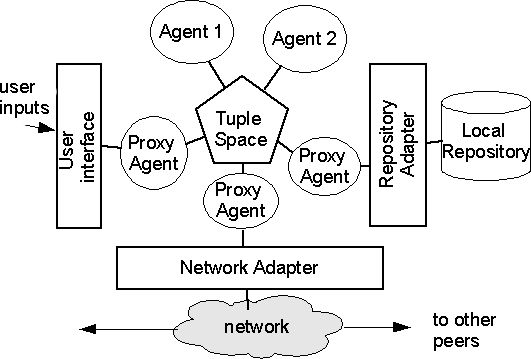
\includegraphics[scale=0.75]{diagrams/U-P2Parchitecture.png}
	\caption{Architecture of U-P2P}
	\label{fig:TSarchitecture}
\end{figure}

%-----------------------------------------------
\subsection{Reusable modules of U-P2P}

The different modules described in the U-P2P architecture above are relatively cleanly decoupled, and available as independent pieces that can be reused in other projects. Here are a few suggestions and guidelines to reuse these different modules.

\subsubsection{Tuple Space Framework}
The Tuple Space framework used in U-P2P is an extension of the lighTS library (lights.sf.net) and is available as the independent project Polyester (polyester.sf.net). Polyester is more than a tuple space. Polyester includes a *fast* tuple-space, with a high level of concurrency. The tuples in the tuple space form a special linked list, such that multiple agents (threads) can concurrently read a single tuple in the list (thus allowing for concurrent ``read" operations over the tuple space). For ``in" and ``out" operations, i.e. the addition or removal of tuples to the list, agents go through the list only locking (i.e. obtaining exclusive access to) one tuple at a time, so that other agents may read other parts of the list.

In addition, a multi-threaded (abstract) Agent is provided, that allows easy implementation of ``service-based" interaction with the Tuple Space. The idea is that the agent stores a list of templates, and associates a specific process to each template. When a tuple appears in the Tuple Space matching a given template, the tuple is read and processed once by the agent. When multiple tuples of interest (i.e. matching the agent's templates) appear faster than the agent can process them, they are queued and processed in the order in which they appear.

Agents can coded as part of a project, and can also be dynamically generated from an XML definition, i.e. an application can load the XML document, and create and activate the agent on the fly.

The Polyester project, as available from polyester.sf.net, includes these features, and an example (toy) application focused on XML matching. 
Requests expressed as XPath expressions are read from the tuple space, and matching documents are output in answer tuples.

\subsubsection{Network Adapter}
The network adapter is based on the JTella library (jtella.sf.net), and can be reused to build a client for Gnutella networks. Code written within the context of UP2P was incorporated to the JTella project.

\subsubsection{Local Repository}
The local repository was built using an early version of the eXist XML database (exist.sf.net). Unfortunately, it has some scalability problems and compatibility problems with the W3C DOM standard, therefore we do NOT recommend reusing our repository module. On the contrary, a replacement for our module would be a welcome improvement.

%==============================================================================
\section{Functional Specification of U-P2P}
\label{sec:functionalspec}

This section provides a functional view of U-P2P. 
The Use Cases of U-P2P, as exposed to a human User, and to a remote peer, are described in detail. In order to give some insight on the decoupling of the modules, ``internal" Use Cases are also presented, showing the functionalities of the different modules relative to one another.
Figure \ref{fig:UseCases} shows a modular view of U-P2P, with the Use Cases offered to the different actors, as well as the Internal Use Cases that describe the module interaction within U-P2P.

\begin{figure}[htb]
	\centering
		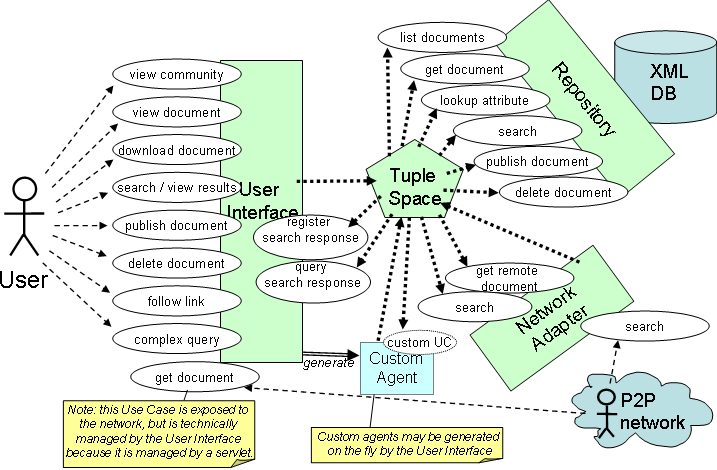
\includegraphics[scale=0.7]{diagrams/modularUseCaseView.png}
	\caption{A Modular View of U-P2P Use Cases}
	\label{fig:UseCases}
\end{figure}

First, section \ref{sec:usecaselist} describes in detail the Use Cases offered to the human user of U-P2P, through its User Interface module, then  section \ref{sec:uclist2} describes the Use Cases offered to the remote peers through the Network Adapter and User Interface. For each of these Use Cases, the module interaction is summarized, as a sequence of Internal Use Cases (see section \ref{sec:moduleinteraction}).

Finally, section \ref{sec:moduleinteraction} details the internal Use Cases where the different modules of U-P2P interact.
For each Use Case, the interaction between modules is described, as a sequence of Tuples written to the Tuple Space and read from it. 

\subsection{Use Cases offered to the local user}
\label{sec:usecaselist} %-----------------------------------------------------------------------------------

\subsubsection{Use Case 1: View Local Document}
\label{uc1}

\paragraph{Summary}
The user can view any document stored in the local repository.

\paragraph{Specification}
The User selects a document from a list (may be a list of search results, or the local contents of a community). The document is shown using the specific rendering style of the community.

\paragraph{Module Interaction}
\begin{figure}[htb]
\centering
	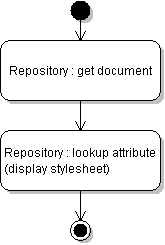
\includegraphics[scale=0.5]{diagrams/uc2-viewdocument.png}
	\caption{UC1, View Document : Activity diagram}
	\label{fig:uc1}
\end{figure}

First the document to be shown is requested from the repository (IUC 1, Repository : Get Document).

Each community may have a specific rendering style for rendering the documents of this community, defined by an XSLT stylesheet, itself an attachment attribute of the community definition document. This XSLT stylesheet, if it exists, must be retrieved next. The document title is also retrieved, which is a two step process: 
	   \begin{enumerate}
	   \item first the standard attribute ``titleLocation" of the community is retrieved, the value of this attribute is the XPath to the title of any document in the community;
	   \item then this community-specific XPath attribute is looked up, and the returned value is the title of the document.
     \end{enumerate}. 

The UI thus outputs the following \emph{Lookup} requests (IUC 3,  Repository : Lookup Attribute, section \ref{iuc3}):
\begin{itemize}
	\item attribute ``community/displayLocation" of the community (i.e. the document \emph{communityId} in the Root Community): this attribute is an attachment and points to the XSLT stylesheet for rendering documents of the community.
  \item attribute ``titleLocation" of the community 
	\item the attribute path returned by the previous request, is looked up for the document to be rendered
\end{itemize} 

The document is then displayed as an XSLT rendering of the XML document, and possibly of attachments (e.g. images) to the document. The result of this XSL transform operation is normally an HTML document.

In the case where the document being viewed is a \emph{community} (i.e. a community definition document), the attributes of the community are shown, not the documents stored in the community. However, an additional link is presented for the user to be able to switch to viewing the community contents.
%--------------------------------------------------------------------------------------------------------------
\subsubsection{Use Case 2: View Community}
\label{uc2}

\paragraph{Summary}
The user can view the list of documents stored in a given community, within the local repository. 

\paragraph{Specification}
The user selects a community displayed in the User Interface, and the documents of this community, stored locally, are listed on the screen. If the community has a specific rendering style, then the collection of documents is shown using this rendering style.
The selected community may be the Root Community, and the list presented is thus the list of communities that the user is a member of. 

\paragraph{Module Interaction}

\begin{figure}[htb]
\centering
	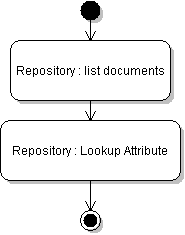
\includegraphics[scale=0.5]{diagrams/uc1-viewcommunity.png}
	\caption{UC2 View Community : Activity diagram}
	\label{fig:uc2}
\end{figure}

First the documents of the community are requested from the Repository (IUC 2 : Repository : List Documents). From the list of documents, an XML tree is built. 

Each community may have a specific rendering style for the collection of its documents, defined by an XSLT stylesheet, as for the individual documents (these are normally two separate stylesheets).

 This XSLT stylesheet, if it exists, must be retrieved next, along with the community Title, which will be displayed on the screen. (IUC 3,  Repository : Lookup Attribute) Retrieving the community Title is the same two-step process as for any document; in this case the first request applies to the Root Community definition document, and thesecond to the document defining the community to be displayed.

The collection of documents is then displayed by an XSLT operation (transformation of the full XML tree using the community display stylesheet).
%---------------------------------------------------------------------

\subsubsection{Use Case 3: Search / View results} 
\paragraph{Summary}
The User searches a community (locally and in the P2P network) for documents matching specific search criteria.

\paragraph{Specification}
The User selects a community, then inputs a search request, using community-specific criteria, through an HTML form. The search request applied to the local repository, and propagated in the P2P network, to other peers members of the community. The responses arrive asynchronously, and are shown on the screen as they arrive. 

\paragraph{Module Interaction}

\begin{figure}[htb]
\centering
	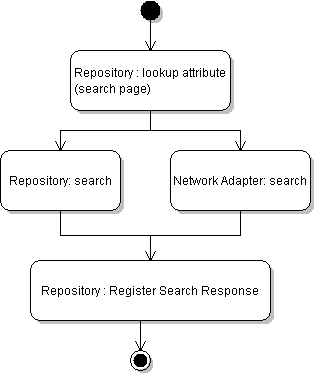
\includegraphics[scale=0.5]{diagrams/uc3-search.png}
	\caption{UC3 Search : Activity diagram}
	\label{fig:uc3}
\end{figure}

The basic search functionality is meant for searching documents of a given community, but within the full P2P network (i.e. within the set of peers that are members of that community). A search form is either automatically generated from the community schema (offering the possibility of filtering documents by attribute values) or is provided with the community definition document. In the latter case, it is retrieved by a \emph{lookup} of the attribute ``community/searchLocation" in the community definition document. (IUC 3,  Repository : Lookup Attribute)

The user inputs her search criteria using the form: valid search criteria consist of conditions over attributes of the documents. 

The search criteria are translated into a single XPath expression, a query identifier is generated to track answers to the query, and the search is output to the Tuple Space. 

A single request is output and is read by both the Repository (IUC4, Repository : Search) and the Network Adapter (IUC7, NetworkAdapter: Search).

The User Interface collects and stores the responses to searches (IUC9, User Interface: Register Search Response), with their metadata. 
A notification is output when each search response is registered : this additional notification allows other modules or agents to query the local collection of search responses *after* they have actually been stored by the UI.

The User Interface presents a ``Search Results" page. The results are listed as a table, and for each result the title, and possibly additional metadata is shown. A link is available to download results from other peers, or to view them (cf. UC2) if they are already found locally.
The page updates automatically to show new results as they arrive: the page repeatedly queries the local collection of search results and updates the results table.

%--------------------------------------------------------------------------------------------------
\subsubsection{Use Case 4: Publish Document.} 
\label{uc4}

\paragraph{Summary}
The User uploads a new XML document, or creates it through a custom HTML form, and the document is stored in the local repository and shown on the screen.

\paragraph{Specification}
The User uploads a well-formed XML document through a file entry form, or else uses a community-specific HTML form to enter the data to compose the XML document. Once submitted, the document is stored in the local repository, then shown to the user using the community rendering style (cf. UC2, view document).

\paragraph{Module Interaction}
\begin{figure}[htb]
\centering
	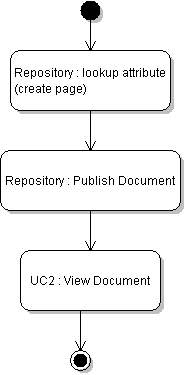
\includegraphics[scale=0.5]{diagrams/uc5-publish.png}
	\caption{UC4 Publish : Activity diagram}
	\label{fig:uc4}
\end{figure}

For each community, a \emph{create form} can be attached to the community definition document. It is then retrieved by a \emph{lookup} of the attribute ``community/createLocation" in the community definition document (IUC3 Repository : Lookup Attribute). If no form is provided with the community, a form is generated from the XML schema of the community.

The form, once submitted, provides the system with a list of key-value pairs from which a new XML document is constructed. Attachments may also be uploaded via HTML \emph{file} form entries. Once the new document is created, it is added to the local repository, and displayed on the screen (cf. Use Case 1).

Alternatively, the create form may be generated automatically from the community schema (if no specific form is provided). The rest of the Use Case is then the same. For complex schemas, automatically generating a schema may be difficult.

The User creates a new resource either by entering its data in a form, and submitting that form, or by selecting a ready-made XML file from her local system. Attachments must be uploaded separately.

The User Interface then publishes the document. This is a three step process:
\begin{itemize}
\item The XML content of the document must be stored in the local repository;
\item The XML file, which is stored on the filesystem, must be mapped to the document in the repository, for implementation-dependent reasons;
\item Any attachments of the document, also stored on the filesystem, must also be mapped to the document.
\end{itemize}

The User Interface generates Tuples containing all three requests and outputs them to the Tuple Space. These requests are not answered, and are simply output in sequence.

For details of the tuples see IUC 4, Repository : Publish, section \ref{iuc4}.
Once the publish requests have been output, the User Interface outputs a request to view the published document (see UC1, section \ref{uc1}), which then appears on the screen.

In the case where the newly published document is a Community Definition Document, the new community (i.e.collection) is added to the Repository.

\emph{Note: in future developments a single tuple should be used in the tuple space, containing all the necessary information. The repository should then handle the different steps of the process.}
%---------------------------------------------------------------------
\subsubsection{Use Case 5: Delete Document} 
\label{uc5}

\paragraph{Summary}
The User removes a document from the local repository.

\paragraph{Specification}
When viewing a community (UC2), a \emph{delete} link is presented next to each document of the community, and the user can click this link to delete the document. The document is only deleted from the local repository. Copies stored by other peers in the network are not affected. If the document is a community definition document, then all the documents locally stored in that community are also deleted.

\paragraph{Module Interaction}

\begin{figure}[htb]
\centering
	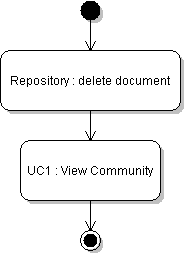
\includegraphics[scale=0.5]{diagrams/uc6-delete.png}
	\caption{UC5 Delete : Activity diagram}
	\label{fig:uc5}
\end{figure}

The request to delete the document is sent to the Repository (IUC6: Repository : Delete Document).

The page is refreshed, showing the community without the deleted resource (UC2). Note that copies of the resource elsewhere in the network are not affected.

In addition, in the case when the deleted resource is a community, all the documents locally stored within that community are deleted (cf. IUC6).

%---------------------------------------------------------------------
\subsubsection{Use Case 6: Download Resource} 
\label{uc6}

\paragraph{Summary}
The User downloads a document from another peer. It is stored locally and shown on the screen.

\paragraph{Specification}
From a list of search results, the user can select a document (not stored locally) and click on a link to download it. The link specifies which peer the document will be downloaded from. An HTTP connection is opened with the remote peer and the document is downloaded to the local system. The document is then stored in the local repository (see UC5, ``publish document"), and shown on the screen.

\paragraph{Module Interaction}
\emph{The following describes the current implementation, which needs to be changed.}
\begin{figure}[htb]
\centering
	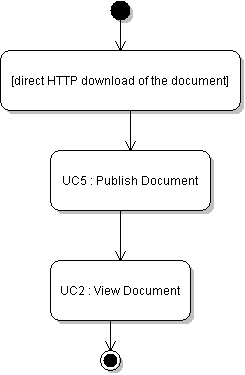
\includegraphics[scale=0.5]{diagrams/uc4-download.png}
	\caption{UC6 Download : Activity diagram}
	\label{fig:uc6}
\end{figure}

Currently, this download is processed by the Network Adapter module, by a direct method call from the User Interface module. This process should go through the tuple space.

Once the file has been retrieved to the local filesystem, it is published and shown on the screen (see Use Case 4, Publish, section \ref{uc4}).

Note that the downloaded document may be a community definition document, in which case the new community is added to the repository in the root community, and the user becomes a member of the new community.

%-----------------------------------------------------------------
\subsubsection{Use Case 7: Follow link } 

\paragraph{Summary}
From viewing a document containing a link to another document, the user navigates to the other document.

\paragraph{Specification}
As described in section \ref{section:concept}, documents can reference one another by links. These links do not point to a document stored by a specific peer, but to \emph{any copy} of a document. When viewing a document A, containing a link to a document B, the user may click on the link in order to search for document B. If document B is stored locally, then it is shown on the screen (cf. UC1), otherwise a search is output for document B in the appropriate community, and the search results page is shown with available copies of document B (cf. UC3).

If the peer is not a member of the community of document B (i.e. the community is not found locally) then a search is output for the community, and the results page is presented, with available copies of this community.

\paragraph{Module Interaction}
\begin{figure}[htb]
\centering
	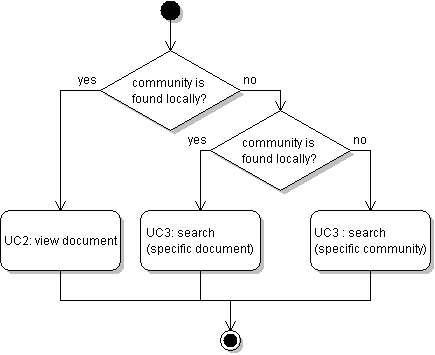
\includegraphics[scale=0.5]{diagrams/uc7-followlink.png}
	\caption{UC7 Follow Link: Activity diagram}
	\label{fig:uc7}
\end{figure}

The User Interface first outputs a lookup request (IUC3 Repository : LookupAttribute) to determine whether the document is available from the local repository. (The lookup request takes the wildcard Xpath selector ``.").
If the document is found locally, then the User Interface outputs a request to retrieve the document and to view it. The processing is then as in Use Case 1.

If the document is not found locally, then a search message is formed where the search criterion is a condition on the document identifier (``resourceId=\emph{value}").

If the community that the document belongs to is not found locally (i.e. the peer is not member of this community) then the previous search is replaced by a search for the community definition document, so that the peer can join the community.

The search requests are processed as in Use Case 3.

%-------------------------------------------------------------------------
\subsubsection{Use Case 8: Complex Query } 

\paragraph{Summary}
The User searches the interlinked documents of the P2P network, using a complex graph query expressed using a specific interface.

\paragraph{Specification}
The graph of interlinked documents can be searched through custom graph queries. The User expresses her query as a graph pattern, using the Query Interface of the UP2P web Interface. A graph pattern is defined as a sequence of links; for each link the direction of the link and the label (XML attribute path) must be indicated. 

Answers to the query are documents, which are then shown in the results page, as for simple searches (UC3).

\paragraph{Module Interaction}

The graph query is decomposed into a sequence of simple subqueries, which can be answered either by simple searches (UC3) or by attribute lookups on the results of the previous subquery (IUC10, Repository : Query Search Response).

These requests are not managed directly by the User Interface ; the User interface creates a set of agents, that each handle one subquery. These agents are deployed to the Tuple Space and started.

The full complex query process, along with its interface, is presented in more detail, with examples, in section \ref{sec:ComplexQueries}.

%--------------------------------------------------------------------------
\subsection{Interaction by remote peers}
\label{uclist2}
Remote peers may also use the system, by submitting search or download requests through the network, and by creating complex queries or following links. 
However, in the network, only simple search messages are seen: complex behavior is broken down into atomic searches or downloads. This allows U-P2P to use traditional P2P protocols such as Gnutella (our built-in protocol in this implementation).
The interface of the U-P2P client with other peers in the network is defined as the format of the messages which are exchanged between peers.
Search and Search Response messages are encapsulated within Gnutella QUERY / QUERYHIT messages \footnote{in previous implementations other protocols were also used \cite{UP2P2002, UP2P2003, UP2P2006}}. Download requests are sent as HTTP requests and managed by a servlet.

Please see Section \ref{Appendix2} for the format of XML Search / Search Response messages, and the specification of the HTTP download requests.

The interaction by a remote peer can thus be described by the handling of search messages and download requests. The following Use Cases describe the system's handling of these messages.
%--------------------------------------------------------------
\subsubsection{Use Case 9: Search request from Network} 
 When a remote peer searches the network (UC3), the search is sent out to all the peers reachable in the network, that are part of the community. This Use Case describes the handling of such a message. 

\paragraph{Summary}
A search message reaches the local U-P2P client, on a listening port. The local repository is searched according to the criteria indicated in the search message, and results are sent back to the remote peer.  

\paragraph{Specification}

This Use Case is triggered by a Gnutella QUERY message received on the network listening port. 
First, at network level, the QUERY message is forwarded to all the peer's other connections (i.e. all the peers that the peer is connected to, minus the peer that sent the message) with a decremented Time To Live (Gnutella protocol).

The search criteria is extracted from the message, and the local repository is searched. The responses are collected and used to compose one or several QUERYHIT messages. The QUERYHIT messages are returned to the peer that the corresponding QUERY message was received from (gnutella protocol).

\paragraph{Module Interaction}

\begin{figure}[htb]
\centering
	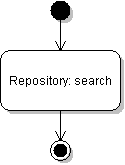
\includegraphics[scale=0.5]{diagrams/uc9-searchfromnetwork.png}
	\caption{Use Case 9 : Activity diagram}
	\label{fig:uc9}
\end{figure}
 
The search criteria and queryId are extracted from the message. The QueryId is stored so that the same query is not processed multiple times. 

The query is submitted to the Repository (IUC4, Repository : Search), and responses are collected by the Network Adapter. The data from the responses, including the XML metadata of matching documents, are placed in one or several QUERYHIT messages. As the QUERYHIT messages are limited in size (set to 64kb in U-P2P), the list of responses may need to be split between multiple messages, and in the case of very large XML files, the XML may need to be truncated.

%--------------------------------------------------------------
\subsubsection{Use Case 10: Download Request from Network}

When a remote peer downloads a resource (UC4), the download request is sent out to the peer storing the resource. This Use Case describes the handling of such a request. 

\paragraph{Summary}
A download request reaches the local U-P2P client system on a listening port. The requested resource is retrieved from the repository and sent to the remote peer.

\paragraph{Specification}
The download request is an HTTP request formatted as follows : 
\begin{verbatim}
http://[IP]:[port]/up2p/community/[communityId]/[documentId]
\end{verbatim}
The IP address is the local peer's IP address, and the port is the listening port of the Tomcat Server (which is different from the Gnutella port).
The \emph{communityId} and \emph{documentId} specify the document to be returned.

An HTTP connection is opened with the requesting peer and the document is sent.

\paragraph{Module Interaction}
This HTTP request is caught by Tomcat, and thus is technically processed by the User Interface.  
Currently, it is not processed through the Tuple Space, but by direct method calls, through the Repository.
\emph{(Note: this should change)}

%================================-------------------------------------
\subsection{Internal Use Cases}
\label{sec:moduleinteraction}

This section describes in detail the tuples exchanged in the tuple space, for each of the ``internal" Use Cases, where the different modules interact.
Each of these Use Cases describes a functionality of a particular UP2P module -- the Repository or the Network Adapter. 
Each Use Case is triggered by tuples appearing in the tuple space : the modules have a list of templates, and permanently listen for matching tuples, which are then processed, and in some cases the module outputs new tuples as a response.

Each of the following internal Use Cases is first briefly specified, then the format of the template triggering the Use Case, and the Response tuples that are output as a result, are given.

\subsubsection{IUC1 : Repository : Get Document}
\label{iuc1}
\paragraph{Specification}
A document, identified by its \emph{communityId} and \emph{documentId} is copied from the repository and returned as an XML DOM object.

\paragraph{Template}
First the document to be shown is requested, by the following tuple:
\begin{equation*}
[\text{``GetLocal"}; communityId; documentId; queryId]
\end{equation*}
The \emph{communityId} and \emph{documentId} identify the document to be retrieved. The \emph{queryId} is no longer used.

\paragraph{Responses}
The Local Repository returns the following (synchronous) response :
\begin{equation*}
[\text{``GetLocalR"}; communityId, documentId; DOM]
\end{equation*}
The \emph{DOM} field contains the requested XML document. Note that this field is of the formal type \emph{XMLField}.

%---------------------------------------------------------
\subsubsection{IUC2 : Repository : List Documents}
\label{iuc2}
\paragraph{Specification} 
All the documents of community \emph{communityId} are listed. Technically, the documents returned are those matching the input XPath expression, i.e. the documents such that the XPath query evaluated against that document returns a non-empty set of nodes. 
Each such document, identified by the pair \emph{(communityId, resourceId)}, is a response.

In this case, the input Xpath is a wildcard matching all the documents, but in the future this parameter can be used to filter documents. 

The Use Case is different from other searches because it is limited to the repository and meant to be synchronous: the list of responses is output atomically (i.e. in a single output operation) to the Tuple Space. This is a necessary condition for synchronicity, as the calling process only reads a single set of responses. Once one or several responses are found, the agent stops listening.

Similarly, if nothing was found, a tuple indicating this must also be output in order to unblock the synchronous listening process.

\paragraph{Template}
\begin{equation*}
[ \text{``SynchroLocalSearch"}; communityId; xPath] 
\end{equation*}
Normally xPath is ``.", which matches any document in the community (i.e. this expression returns the root node of the document, which is always a non-null result). However in the future this could be used to filter documents.

\paragraph{Responses}

For each pair \emph{(communityId, resourceId)}, a response tuple is output with the following format:
\begin{equation*}
[ \text{``SynchroLocalSearchResp"}; communityId; xpath; resourceId]
\end{equation*}

If nothing was found, the following tuple is output :
\begin{equation*}
[ \text{``SynchroLocalSearchResp"}; communityId; xpath; \text{``"} ] 
\end{equation*}

%---------------------------------------------------------
\subsubsection{IUC3 : Repository : Lookup Attribute}
\label{iuc3}
\paragraph{Specification}
The request specifies a document, through the identifiers \emph{(communityId, resourceId)} and an attribute, defined by the XPath expression \emph{xpath}). 
The repository returns the string value for this attribute in the specified document, or a list of values if the attribute is multi-valued.

Note: this call is synchronous, and the answer tuples must be output atomically.

\paragraph{Template}
In the Tuple Space, a lookup request is formatted as follows: 
\begin{equation*}
[\text{``LookupXpath"}; documentId; communityId; xpath]
\end{equation*}

\paragraph{Responses}

For each response, a tuple of the following format is output:
\begin{equation*}
[\text{``LookupXpath"}; documentId ; communityId; xpath ; answer]
\end{equation*}
One such tuple is output for each answer (i.e. for each value of the requested attribute in the specified document).

If an error occurs, the Repository returns one of the following tuples, depending on the error:
\begin{eqnarray*}
[\text{``LookupXpath"}; documentId ; communityId; xpath ; \text{``CommunityNotFound"]} \\  \text{[``LookupXpath"}; documentId; communityId; xpath; \text{``ResourceNotFound"}] 
\end{eqnarray*}

%----------------------------------------------------------------------------------
\subsubsection{IUC4 : Repository : Search}
\label{iuc4}
\paragraph{Specification}
The Local Repository evaluates the input XPath query over documents stored locally, and outputs a response tuple for each matching document. 
A matching document is a document such that the XPAth query evaluated against the document returns a non-empty set of nodes.

\paragraph{Template}
A search request tuple has the following format:

\begin{equation*}
[\text{``SearchXpath"}; communityId; xPath; queryId]
\end{equation*}

\paragraph{Responses}
Search Response Tuples have the following format:
\begin{eqnarray*}
[\text{``SearchXpathAnswer"}; communityId; documentId; title; \\ filename; location; queryId; DOMmetadata]
\end{eqnarray*}

The \emph{documentId} identifies each response document, and the \emph{title}, \emph{filename}, are other attributes of this document. The \emph{DOMmetadata} is the pure XML content of this document (without attachments and limited in size, used for filtering and looking up attributes of search responses). The \emph{location} is an HTTP link to download the file. Note that there may be multiple responses for a given file, with different locations.

%----------------------------------------------------------------------------------

\subsubsection{IUC5 : Repository : Publish Document}
\label{iuc5}
\paragraph{Specification}
a Publish operation requires three different steps:
\begin{itemize}
\item The XML content of the document must be stored in the local repository;

The repository stores the document represented by the XML tree \emph{DOM} in the community \emph{communityId} with the identifier \emph{documentId}. 

\item The XML file, which is stored on the filesystem, must be mapped to the document in the repository, for implementation-dependent reasons;
The corresponding tuple is interpreted as : the file \emph{filepath}\footnote{The \emph{filepath} is simply the filename, and no longer the full path to the file, as in previous implementations. Documents and attachments are stored in standardized directories, which improves portability: the full U-P2P directory on the filesystem can be copied or moved without any problems.} is mapped to the document identified by \emph{communityId} and \emph{documentId}. 

\item Any attachments of the document, also stored on the filesystem, must also be mapped to the document.
The file \emph{filename} is an attachment of the document \emph{documentId}, identified within this document by the attachment name \emph{attachname}.

\end{itemize}


\paragraph{Template}
Currently, a publish operation requires three separate tuples.

A publish request is formatted as follows:
\begin{equation*}
[\text{``PublishXML"}; communityId; documentId; DOM]
\end{equation*}

Document mapping requests are formatted as follows:

\begin{equation*}
[\text{``MapFile"}; communityId; documentId; filepath]
\end{equation*}

Attachment mapping requests are formatted as follows:

\begin{equation*}
[\text{``MapFile"}; communityId; documentId; filepath; attachname]
\end{equation*}

\paragraph{Responses}
No responses are output to this request.

%----------------------------------------------------------------------------------
\subsubsection{IUC6 : Repository : Delete Document}
\label{iuc6}
\paragraph{Specification}
The specified document is deleted from the local repository. 

\paragraph{Template}
The User Interface outputs a tuple to the Tuple Space with the following format:
\begin{equation*}
[\text{``Remove"}; communityId; documentId]
\end{equation*}
The identifiers \emph{communityId} and \emph{documentId} indicate which document is to be removed.

\paragraph{Responses}
If an error occurs, a tuple is output to the tuple space, containing the error message:
\begin{equation*}
[\text{``NotifyError"}; errormsg]
\end{equation*}

%----------------------------------------------------------------------------------

\subsubsection{IUC7 : Network Adapter : Search}
\label{iuc7}
\paragraph{Specification} The Network Adapter encapsulates the query in a Gnutella QUERY message and outputs it to the network. It then collects responses (which come in QUERYHIT messages), extracts the relevant data and places this data in Search Response Tuples.
Note : this call is asynchronous, and answers may come in sequence at any time.

\paragraph{Template, Response}
The Template and Response format are the same as in the Repository Search, see section \ref{iuc4}.

%----------------------------------------------------------------------------------
\subsubsection{IUC8 : Network Adapter : Get Document}
\label{iuc8}
Currently this operation does not go through the tuple space, but through direct method calls (should be changed).
%\paragraph{Template}
%\paragraph{Process}
%\paragraph{Responses}

%----------------------------------------------------------------------------------

\subsubsection{IUC9 : User Interface : Register Search Response}
\label{iuc9}
\paragraph{Specification}
Each time a search response tuple appears in the tuple space, it is registered by the User Interface, and its XML metadata is stored so that it can be queried by other processes. 

A copy of the input tuple, without the XML metadata, is then output. This tuple serves as a notification to other processes, that the corresponding search response has been registered and that the DOM metadata can be queried (see IUC10, below).

\paragraph{Template}
The User Interface collects all searchresponses with the following format (output by IUCs 4 and 7, see sections \ref{iuc4} and \ref{iuc7}).
\begin{eqnarray*}
[\text{``SearchXpathAnswer"}; communityId; documentId; title; \\ filename; location; queryId; DOMmetadata]
\end{eqnarray*}

\paragraph{Responses}
The User Interface outputs tuples of the following format:
\begin{eqnarray*}
[\text{``SearchXpathAnswer"}; communityId; documentId; title; \\ filename; location; queryId]
\end{eqnarray*}

Note that the only difference with the input tuples are the lack of DOMmetadata. 

%----------------------------------------------------------------------------------
\subsubsection{IUC10 : User Interface : Query Search Response}
\label{iuc10}
\paragraph{Specification}
The metadata of search responses, stored by the User Interface, can be queried for attribute values.
The input tuple specifies a document and an attribute (as an XPath expression), and the corresponding attribute value is returned. If the attribute is multi-valued, multiple tuples are returned.  

\paragraph{Template}
Request tuples have the following format :
\begin{equation*}
[\text{``LookupSearchResponse"}; documentId; communityId; xpath, queryId]
\end{equation*}

Note: the queryId is no longer used.

\paragraph{Responses}

Response tuples have the following format :
\begin{equation*}
[\text{``LookupSearchResponseAnswer"}; documentId; communityId; xpath, answer, queryId]
\end{equation*}

In the case where no answers were found, the following tuple is output:
\begin{equation*}
[\text{``LookupSearchResponseAnswer"}; \text{``"}]
\end{equation*}

Note : should be changed to include the details of the query.


%======================================================================================

\section{Design of the User Interface}
\label{sec:UIDesign}

\subsection{Overview of the User Interface}

The User Interface of U-P2P is designed as a JSP-based Web Application. The general principle of this design is that the Interface itself is composed of different JSP (Java Server Pages) that offer an HTML-type interface, with forms and links, and through these forms and links invoke active behavior coded in the JSP pages themselves, in Tags embedded in the JSPs, and separate Servlets.

Below this purely ``web-oriented" interface is the part of the interface that implements the U-P2P internal logic, including the interaction with the Tuple Space. This part of the interface can be invoked through a non-web interface, such as a java console (see section \ref{sec:consolemode}). 

Figure \ref{fig:UIOverviewClasses} illustrates this design.

\begin{figure}[htb]
\centering
	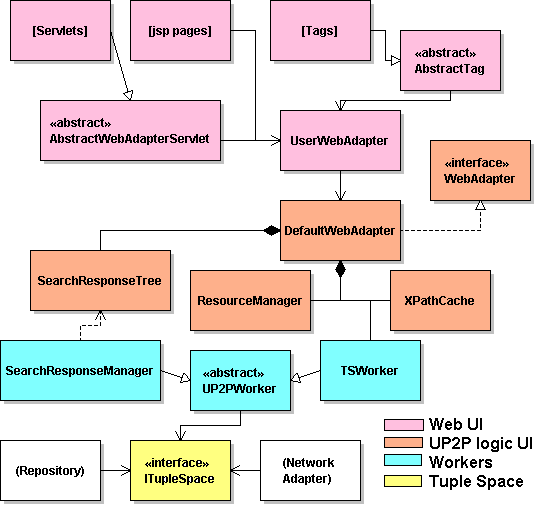
\includegraphics[scale=0.5]{diagrams/UP2PUserInterfaceClassesColor.png}
	\caption{UP2P User Interface : class diagram}
	\label{fig:UIOverviewClasses}
\end{figure}

In section \ref{sec:WebUI} we will describe the web-oriented part of the interface, namely the JSP pages, Tags, and Servlets.

In section \ref{sec:defWebAdapter} we will cover the classes implementing this functional layer of the User Interface.

\subsection{U-P2P Web Interface}
\label{sec:WebUI}
The U-P2P Web Interface relies on an Apache Tomcat Web Container, which manages the http session and links together dynamic display pages with active code implemented in servlets.

The Web Application is basically a collection of servlets and java objects which are used by these servlets, plus in this case JSP pages which provide interaction with an end user through a web browser. Note that the Tomcat architecture imposes the java core of the application to be one such java object, used by the servlets, which is a bit of a counter-intuitive perception of the application and its user interface.

The Web Container (Apache Tomcat) receives the http requests from the browser and invokes different servlets to handle the requests, according a mapping defined in a configuration file. (For details of the configuration see section \ref{sec:config})

The HTTP requests include parameters which are passed to methods defined in the servlets. The servlets in turn interact with the pure java core of the application. 
JSP pages include java code and may also interact with the application core, as well as with the servlets, to which they can direct requests.

JSPs are HTML documents containing special ``JSP" Tags, which incorporate Java code, either directly in the document, or (at compilation time) from external ``Tag" classes. When a JSP page is deployed, the servlet container generates Java source code from the text and tags, then compiles the source to create servlet classes. The JSP servlet classes are then used to service requests the same way as standard servlets. JSPs generate httpRequests and Responses which are serviced either directly or forwarded to other [jsp or not] servlets. 

Web Components (servlets and JSPs) store additional java objects in PageContext or ServletContext objects managed by the Web Container.
The PageContext stores objects specific to each JSP/Servlet (e.g the request and response), whereas the ServletContext stores objects which are common (global) to the entire Web Application. As mentioned previously, the entire P2P client is materialized here as an object stored by the ServletContext. 

The Web Container uses a RequestDispatcher to redirect processing from one class to another, and carries the data through httpSession attributes, and httpServletRequest / Response objects are the actual arguments of redirection methods. This way, any processing is initiated by an http request sent from the browser, and finalized by an httpResponse.

Figure \ref{fig:WebUI} shows the interaction between the JSP pages, the tags embedded in these pages, and the Servlets.

\begin{figure}[htb]
\centering
	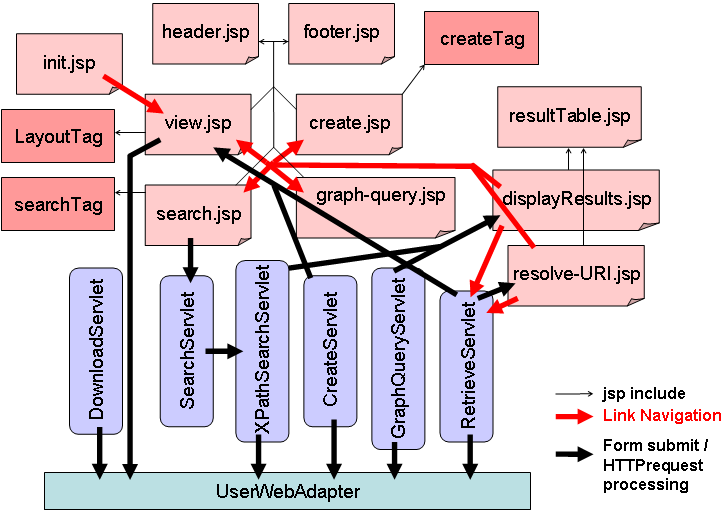
\includegraphics[scale=0.5]{diagrams/JspsAndServlets.png}
	\caption{UP2P Web Interface : JSPs and Servlets}
	\label{fig:WebUI}
\end{figure}

%--------------------------------------------------------------------------------------------------------------------
\subsubsection{JavaServer Pages}

\begin{itemize}
\item \textbf{header.jsp} Included as the header for all JSPs that use the layout tag. It displays links to all the communities known to the user and links for the three activities of View, Search and Create.

\item \textbf{footer.jsp } Included after the body for all JSPs that use the layout tag.

\item \textbf{disabled.jsp } Prevents the user from attempting to search or create resources where there is no Network Adapter available for the community. Once the correct Network Adapter is installed, this page will no longer be displayed. Triggered from the networkadapter-check taglib on the search.jsp and create.jsp pages.

\item \textbf{create.jsp } Uses the create-page tag to display the create page for a community. Forms are either submitted to UploadServlet for uploading files or CreateServlet for creating resources with an HTML form.

\item \textbf{search.jsp } Uses the search-page tag to display the search page for a community. Searches are submitted to the SearchServlet.

\item \textbf{upload.jsp } Included by the create-page tag to allow users to upload prepared XML resources.

\item \textbf{overwrite.jsp } Displayed when a duplicate resource is uploaded.

\item \textbf{schemaTool.jsp } Links to SchemaTool.

\item \textbf{community-create.jsp } Used by the Root Community Create screen to allow for dynamic configuration of Network Adapters. The Root Community is a special case because Network Adapters have to be configured when manually creating a community. Normally, communities would have a static HTML create page.

\item \textbf{displayResults.jsp } Retrieves the search results stored in the Servlet context (at the application scope) and displays them in a table for the user. Download links direct the user to RetrieveServlet.

\item \textbf{init.jsp } Used to display information when U-P2P is initialized.

\end{itemize}
%------------------------------------------------------------------------------------
\subsubsection{Tags}
Tags are used to display dynamic content in jsp pages through pure java code which can be called anytime by simple markup tags, such as the tag \\ \verb.<up2p:create-page>., found in the create.jsp page. 
Calling tags to display content is handled by the Web Container. The available tags are defined in the tag library <taglib> defined in the file WEB-INF/up2p-taglib.tld
The jsp tag \verb.<up2p:create-page>., for instance, is implemented by the CreateTag.java class, as described in the tld:
\begin{verbatim}
<tag>
 	<name>
 			create-page
 	</name>
  <tag-class>
   		up2p.jsp.CreateTag
  </tag-class>
  <description>
   		Renders the U-P2P create interface for a community.
  </description>
</tag>
\end{verbatim}

The class which implements the tag contains code to be executed at the opening tag, in the method doStartTag() and at the closing tag, in the method doEndTag(). 

U-P2P requires that dynamic pages be served up to the user for such activities as Search, Create and View. The general flow of events that occur in one of these activities involves the user accessing a JSP, the JSP submitting a form to a Servlet and the Servlet talking to the WebAdapter and then returning to a JSP.

Figure 3 shows the pages and Servlets involved in each activity as well as the two extra Servlets needed for diagnostic reasons and for servicing download requests.

\paragraph{Tags in U-P2P}
\begin{itemize}
\item \textbf{AbstractTag} Abstract class for all the U-P2P tags.
\item \textbf{CreateTag} Lays out the form on the create page using the specific display for a community.
\item \textbf{LayoutTag} Implements the layout of the JSP pages. Inserts headers and footers, sets parameters, retrieves stylesheets according to display mode (search, create, view).
\item \textbf{SearchTag} Implements the JSP tag for the search page.
\end{itemize}
%------------------------------------------------------------------------------------
\subsubsection{Servlets}
Note: The current community ID is now stored in the user session and used throughout the JSP pages. The name of the session attribute is defined as \verb;AbstractWebAdapterServlet.CURRENT_COMMUNITY_ID;.

\begin{itemize}
\item \textbf{CreateServlet} Forms an XML document from the submitted HTML form and submits it to the UploadServlet. Creating an XML document from form parameter/value pairs is no easy task, so this Servlet requires that the parameters are simple XPaths pointing into the document to be created and parameter values are populated into the new document.
The XPaths must explicitly be slash-separated path values (e.g. book/title) with no function calls or predicates. See http://www.w3.org/TR/xpath for details on Xpath. 

For example, to create the following instance document:
\begin{verbatim}
<book>
<title>Serpent of Nigara</title>
<author>J. M. Doolittle</author>
</book>
\end{verbatim}

The form would submit the following parameter/value pairs:

book/title=Serpent of Nigara\\
book/author=J. M. Doolittle

This would result in the correct XML structure being created and the resulting document would be first written to disk under the community folder, and the response is redirected to the UploadServlet for processing and publishing.

Additionally, the \verb.up2p:filename. parameter is required (all parameters starting with up2p: are not included as XPaths) and special functions are supported for creating dates and inserting attachment information. 

%\begin{itemize}

\item \textbf{UploadServlet} Takes a file specified in the up2p:filename parameter and after processing, sends it to the WebAdapter for publishing (where it is stored in the database and published on the network). In the WebAdapter the file is checked for XML validity and its ID is generated using a hash function.

\item \textbf{SearchServlet} Constructs searches and sends them to the XpathSearchServlet (and indirectly to the WebAdapter and then on to the Network Adapter). The searches are formed as in CreateServlet, with parameter names as XPaths and values as case insensitive keywords that should be found at that XPath. None of the special parameters of the CreateServlet are supported. This search format is intended to be a generic XML XPath query that will eventually be replaced by the more complex standard, XML Query (W3C Working Draft).

A complete search query is composed by taking each XPath and adding the value to the end in a predicate form. Each XPath expression is then combined using a Boolean AND operation and the final query is sent to the WebAdapter.

\item \textbf{XpathSearchServlet} Accepts a complete XPath query in the up2p:XPathSearch parameter and sends the search to the WebAdapter. The XPath must be well formed or the search will be rejected.

The results of a search are stored in an attribute of the user session. After submitting the search form, the servlet will perform the search, store the results as an array of SearchResponse objects in the user session and then redirect the user to displayResults.jsp.

\item \textbf{DatabaseViewer} Provides a dump of the repository database listing resources and the file map. The viewer is used by going to http://localhost:8080/up2p/database.xml or http://localhost:8080/up2pserver/database.xml. Currently, this servlet is only used for diagnostis purposes.

\item \textbf{DownloadServlet} Services requests by other U-P2P users to download a particular resource or attachment. This Servlet is mapped to /up2p/community/* so it catches all requests within the community folder.

\end{itemize}

%--------------------------------------------------------
\subsection{User Interface UP2P logic}
\label{sec:defWebAdapter}

For a class diagram of the classes described here, see Figure \ref{fig:UIOverviewClasses}

The central element of this functional module is the \verb.DefaultWebAdapter.. The class name doesn't provide many clues of its purpose, but basically it implements the UP2P internal logic, in terms of User Queries.

User queries are input from the \verb.UserWebAdapter. and passed on to the tuple space. 

The \verb.XPathCache. class caches attribute value lookups, in order to reduce back-and-forth queries for attributes that are used many times. The cache is selectively cleared when documents are removed from the Repository.

The \verb.ResourceManager. class is a legacy class that is used for attribute lookups. It exposes a number of hard-coded \verb.get().-like methods, and answers such requests using a general-purpose ``lookup" method, where the attribute path is a parameter. This lookup is first attempted on the \verb.XPathCache., and if no value is found, it is passed to the Tuple Space to be answered by the Repository.

The \verb.SearchResponseTree. is a temporary repository to store the metadata from remote documents, which comes with Search Responses from the network.
The SearchResponseManager is an agent that collects such responses from the Tuple Space, and also responds to queries over this metadata.
 
%======================================================================================
\section{Design of the Local Repository}
\label{sec:RepositoryDesign}

A class diagram of the local repository is shown in Figure \ref{fig:repositoryClass}.

\begin{figure}[htb]
\centering
	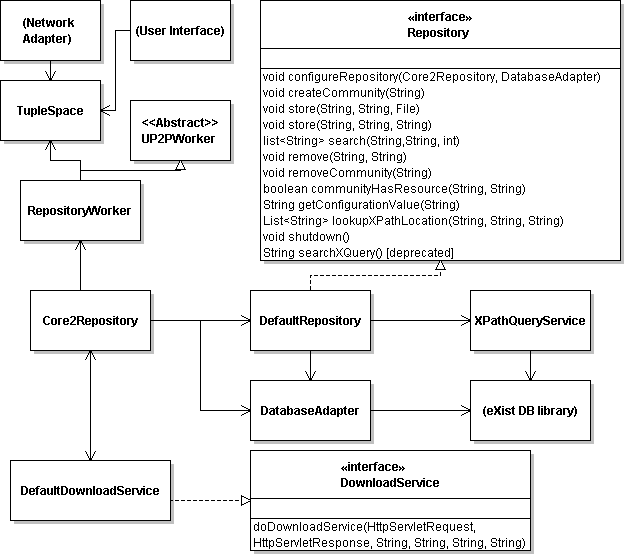
\includegraphics[scale=0.5]{diagrams/UP2PRepositoryClasses.png}
	\caption{Local Repository Module : class diagram}
	\label{fig:repositoryClass}
\end{figure}

%======================================================================================
\section{Design of the Network Adapter}
\label{sec:NetworkAdapterDesign}

The following class diagram (figure \ref{fig:NAClass}) shows the class design of the Network Adapter Module.
\begin{figure}[htb]
\centering
	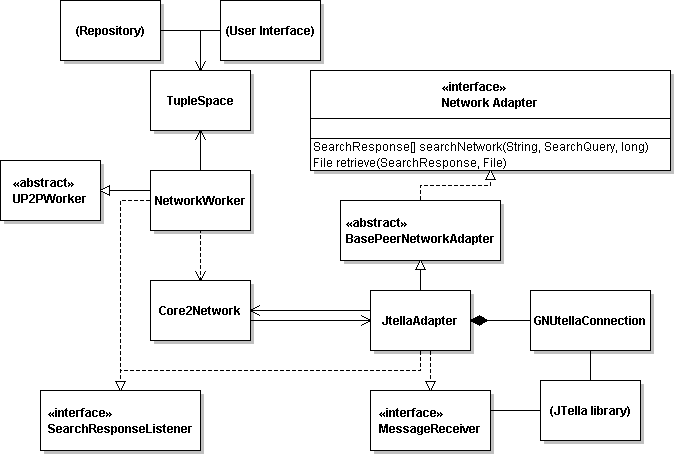
\includegraphics[scale=0.5]{diagrams/UP2PNetworkAdapterClasses.png}
	\caption{Network Adapter Module : class diagram}
	\label{fig:NAClass}
\end{figure}

The network interaction uses the Gnutella protocol, which is implemented in the JTella library. For documentation of the JTella library itself, see \cite{jtellaDoc}.


%======================================================================================
\section{Design of the Tuple Space Framework}
\label{sec:TSDesign}

The Tuple Space Framework includes the Tuple Space itself, and a number of ``agents", or ``workers" that interact with the Tuple Space. These workers include proxies for the different modules and additional workers.
Figure \ref{fig:TSClass} shows a zoom of UP2P class diagram on the Tuple Space.
\begin{figure}[htb]
\centering
	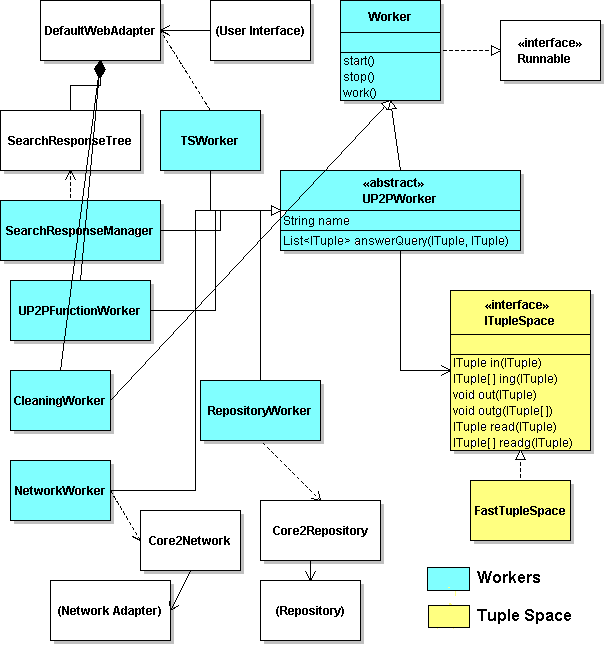
\includegraphics[scale=0.5]{diagrams/UP2PTupleSpaceModuleClassesColor.png}
	\caption{Tuple Space Overview: class diagram}
	\label{fig:TSClass}
\end{figure}

\paragraph{Proxy Agents}
The workers \verb.TSWorker., \verb.SearchResponseManager., \verb.RepositoryWorker., and \verb.NetworkWorker. are ``proxy agents" respectively for the User Interface Module, for the SearchResponse storage module of the User Interface, for the Repository, and for the Network Adapter.

Their purpose is to interface these modules with the Tuple Space, which serves as a coordination middleware between them.

\paragraph{Other Agents}
The \verb.CleaningWorker. is a specialized worker that ensures that tuples do not accumulate in the tuple space. This worker registers the tuples as theyu appear and removes them after a short lifetime in the Tuple Space (configurable).

The \verb.FunctionWorker. is an special worker that supports ``programmed" agents. (see section \ref{sec:AgentProgramming})
This worker responds to a few queries to manipulate strings, specifically string concatenation and parsing of up2p URIs, which cannot be done easily in programmed agents.


Figure \ref{fig:FastTS} shows the design of UP2P's FastTupleSpace.

\begin{figure}[htb]
\centering
	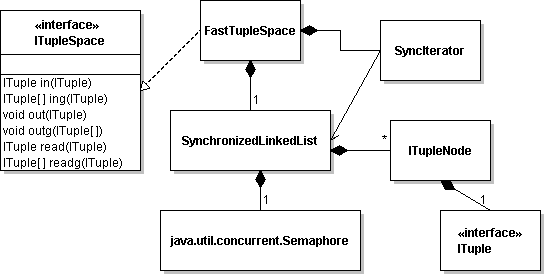
\includegraphics[scale=0.5]{diagrams/UP2PTupleSpaceClasses.png}
	\caption{U-P2P's Fast Tuple Space in detail}
	\label{fig:FastTS}
\end{figure}

The Agents mostly inherit from the abstract class \verb.UP2PWorker.. The \verb.UP2PWorker. is designed for a particular interaction model, where an agent reacts to a collection of templates, each of which triggers a particular process.

This agent model was designed for the following requirements :
\begin{itemize}
\item all templates have equal priority
\item tuples must be processed in the order that they appear in the tuple space
\item no tuple shall be missed
\item tuples must be read and not removed from the tuple space, but should only be processed once
\end{itemize}

Our agents are designed as shown in the class diagram of Figure \ref{fig:TSWorkerClass}.
\begin{figure}[htb]
\centering
	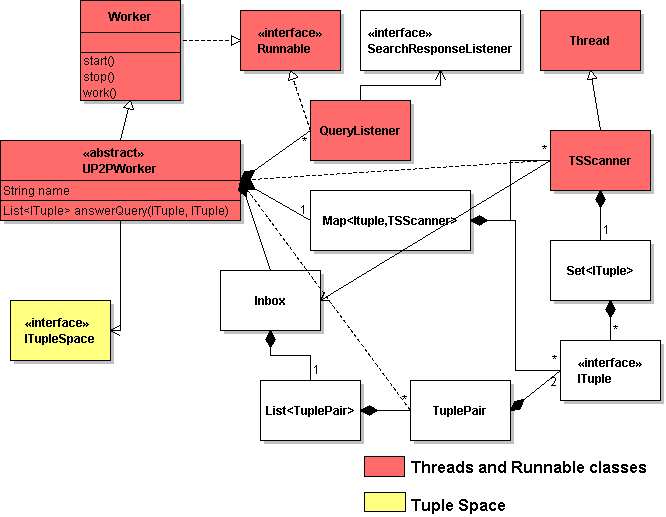
\includegraphics[scale=0.5]{diagrams/UP2PTSWorkerClassesColor.png}
	\caption{UP2P Tuple Space Workers}
	\label{fig:TSWorkerClass}
\end{figure}

The interaction model between a proxy agent and the Tuple Space is illustrated in Figure \ref{fig:WorkerInteraction}.
\begin{figure}[htb]
\centering
	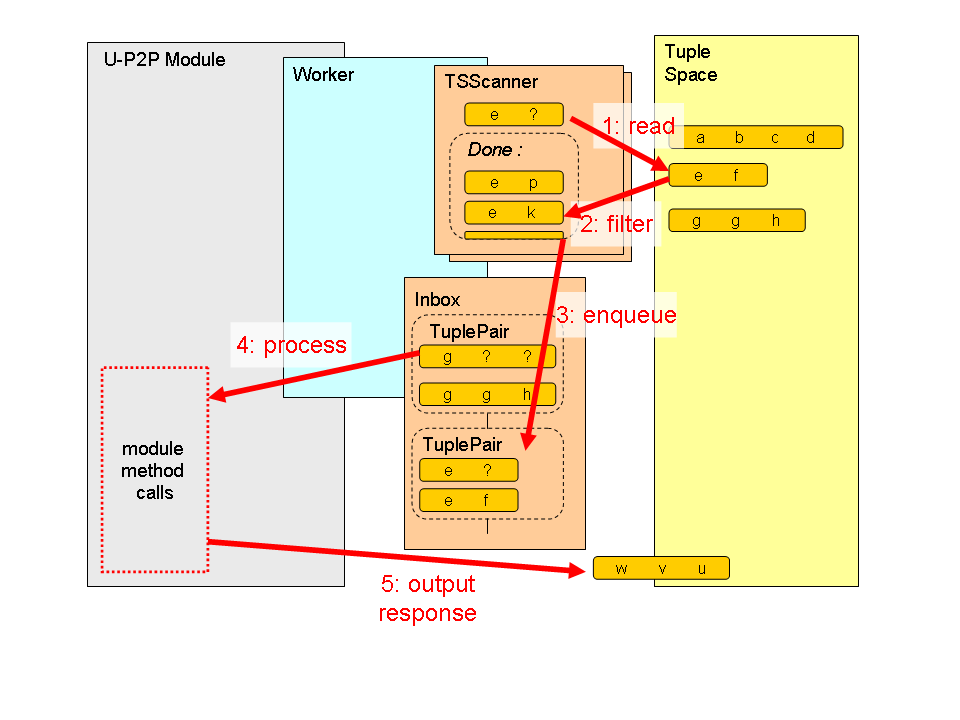
\includegraphics[scale=0.4]{diagrams/WorkerInteraction.png}
	\caption{UP2PWorkers : basic interaction model}
	\label{fig:WorkerInteraction}
\end{figure}

Each \verb.TSScanner. has its own thread, and when new tuples appear in the Tuple Space, the scanners concurrently read them.
The new tuples are first filtered against a list of previously read tuples. 

The filtering is as follows:
\begin{itemize}
\item The list after filtering contains the same tuples that were read in the tuple space (before filtering)
\item The tuples that are kept to be processed are the tuples that were read in the tuple space minus those found in the initial list.
\end{itemize}

The tuples that are kept for processing are enqueued FIFO in the Agent's \verb.Inbox.. The queued contains \verb.TuplePair. objects containing both the Tuple to be processed, and the Template that it matched. The template may be necessary as some tuples could match multiple templates and require to be processed by all corresponding processes (i.e. the processes associated with the templates).

The \verb.Worker. dequeues the \verb.TuplePair.s for processing, and returns a list of response tuples (the list may be empty) to the Tuple Space.

%=======================================================================================
\section{Complex Queries}
\label{sec:ComplexQueries}

The complex query feature of UP2P is the most technical and experimental at this point.

As this guide is under construction at the moment we refer the reader to chapters 5 through 7 of A. Davoust's M.A.Sc. thesis \cite{alanMASCthesis} for the theory and query answering algorithms of these graph queries. 

%======================================================================================
\section{Extensions and Tools}
\label{sec:ExtensionsDesign}

\subsection{Database Initializer}

The \verb.DatabaseInitializer. directly writes the database files of U-P2P, using the configuration files and XML documents in the directory \verb.up2p/data/init..

The database should be initialized (or re-initialized) if U-P2P fails to start due to errors in the database (or a database that has never been initialized). The eXist database is particularly error-prone when heavily loaded.

Note that an alternative to re-initalizing the database is keeping a backup copy of the repository files (entire \verb.data. directory), and simply replacing them and restarting U-P2P (the files must be switched after shutting down U-P2P). 

\subsection{Database Dumper}

In order to troubleshoot the database, the \verb.DBDumper. can also be used to dump the contents of the DB to a file.

\subsection{Console Mode}
\label{sec:consolemode}
As indicated in the section about the User interface, the UP2P User Interface (the ``internal logic" part) can be accessed by a non-web interface.
The UP2P Console mode is an implementation of UP2P as a standalone Java Application.

This mode is not made for elegant rendering of documents, but rather as a tool for processing data-oriented queries or debugging.

The architecture of UP2P deployed in console mode is shown in the class diagram of Figure \ref{fig:UP2PConsoleGUIClasses}.
\begin{figure}
	\centering
		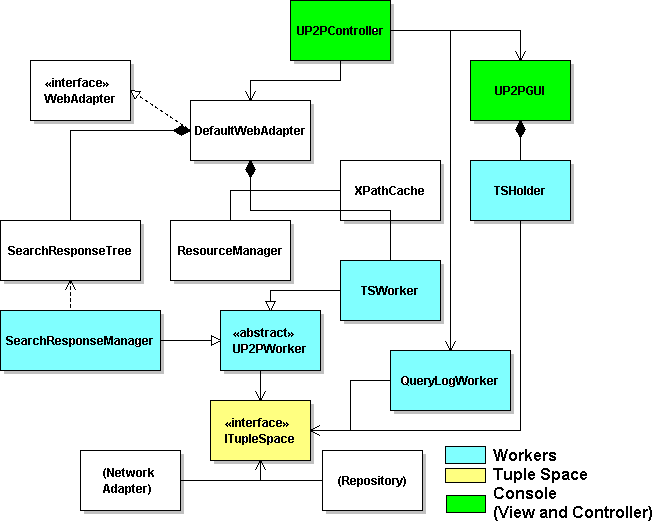
\includegraphics[scale=0.5]{diagrams/UP2PConsoleGUIClassesColor.png}
	\caption{UP2P Console Mode : Class Diagram}
	\label{fig:UP2PConsoleGUIClasses}
\end{figure}

This architecture implements the Model-View-Controller pattern, where the model is the U-P2P internal logic, and the view is provided by a Swing GUI.

The worker \verb.TSHolder. is part of the GUI and provides a view inside the Tuple Space. The other worker that appears in this mode is a QueryLogger, that is meant to be used to run complex query experiments. This worker logs queries and their response times to a file.

\subsection{Agent Programming}
\label{sec:AgentProgramming}

The Tuple Space framework has an experimental extension for \emph{programming} agents.

The behavior of an agent can be specified as a set of rules, following the idea ``when tuple A appears, extract the third field and place it in the second field of template B, then output the resulting tuple". We have defined a schema for encoding such rules in XML, and provide a method to generate an agent automatically from the XML document, i.e. a compiler for this XML-based language.

This compiler is implemented in the class \verb.UP2PAgentFactory., and produces instances of \verb.BasicWorker..

Each rule is formed by a \emph{Head}, which is a template matching tuples that will activate the rule, and a \emph{Tail}, which is a sequence of tuple-instructions (tuple inputs and outputs) to be executed when the rule fires. Each tuple-instruction is a basic Linda operation specifier (in / out / read) followed by a tuple definition.

These tuples only contain String fields, and may include variables: input instructions (in or read) are defined by templates, and the fields of the tuples that match these templates are bound to variables that can be reused in subsequent instructions.

The variable binding process is based on the concept of formal fields, to which we add a variable name instead of a value. In order to reuse a variable, we use what we call ``variable" fields, which will appear at runtime to be literal fields, but whose values are filled in dynamically from stored variables. For example, a formal field bound to variable $x$ will allow us to read a value and store it in the variable $x$, whereas a field declared as a \emph{variable} field will be filled at runtime with the current value for $x$.

A single agent may have multiple rules sharing the same set of variables, and this avoids the need of loop constructs or condition statements, since the former can be replaced by a short rule which can be triggered repeatedly, and a conditional fork can usually be replaced by two rules triggered by the two alternative inputs of the condition.

In order for the execution of an agent to have a meaningful effect in the P2P file-sharing system, the tuples output by agents should match the templates of the permanent U-P2P modules.

Finally, we note that we have added a functionality to lookup metadata values from search responses: The user interface temporarily stores search responses and answers XPath queries over the metadata values of the documents returned in the search.

This abstract ``Agent Definition Language'' can be represented by a schema. Figure \ref{fig:AgentDefLanguage} shows a diagram representing this schema.

\begin{figure}[htb]
	\centering
		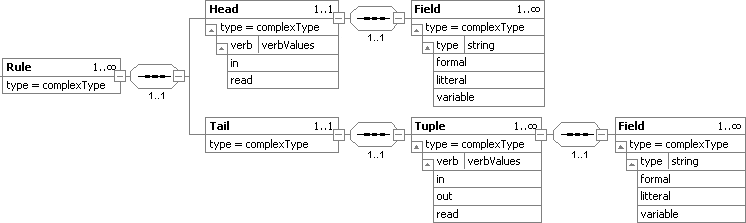
\includegraphics[width=1.00\textwidth]{diagrams/AgentDefXSDdiagram3.png}
	\caption{Schematic representation of the Agent Definition Language.}
	\label{fig:AgentDefLanguage}
\end{figure}


%======================================================================================
\section{Configuration And Testing}
\label{sec:ConfigTesting}
To be done.
%===========================================================================================
\appendix
\newpage
\section{Appendix: suggested improvements to UP2P}

UP2P is still in a development process and there is lots of room for improvement. Here are a few things that need to be done.

\begin{itemize}
\item Modify downloader (client side) to allow for parallel downloads from multiple sources
\item Modify downloader (server side) to go through the Tuple Space. (method ``retrieveFromNetwork")
\item Add a ``stop search" message to stop searches: When the user writes a new search we may assume that the previous search can be called off. JTella provides a method to close search sessions.
\item Add a template for ``NotifyError" tuples, so that the UI notifies the user about errors. Generalize the usage of ``NotifyError" tuples for all use cases. A dialog box should appear notifying the User of the error.
\item Modify the ``publish" process so that it can be done in a single tuple space request. The ``mapfile" requests don't need to be separate calls, all the info can go in a single request tuple.
\item Improve the automatic form generation (from an XSD schema generate an HTML \emph{search} form, a \emph{create} form. Existing methods don't work for complex schemas (of any depth greater than 1), and do not provide the interaction to create multiple values. 
\item Improve the automatic XML document generation from HTML parameter pairs: multi-valued attributes are not supported, and the order of parameters is not maintained on upload. A workaround for this problem would be good.
\item For the console mode, an simple http server needs to be added to service downloads requested by remote peers.
\item Known bug (minor) : Synchronous multi-queries (queries with multiple results) don't always work because if they are repeated in close succession, sometimes the results of the previous request are still in the tuple space, but in the process of being removed by the cleaner agent. In this case the sync call only returns part of the answers (the answers of the previous call, that the cleaner agent has not yet removed).
The solution would be to provide a tuple-space operation ``in" with multiple templates, so that the cleaner agent can remove a set of tuples in a single pass.
\item LookupSearchResponse queries, when no answer is found, return a single tuple 
\begin{equation*}
[\text{``LookupSearchResponseAnswer"}; \text{``"}]
\end{equation*}
This should be changed to something more specific to the query.
\item The Repository Interface has a method for XQuery queries. This method is called by direct method calls from XQueryServlet-UserWebAdapter-DefaultWebAdapter-Core2Repository-Repository.
The XQuery servlet is not currently used, but the code is still present.

We need to determine whether to make use of the XQuery servlet -- and in this case implement the calls through the Tuple Space, or to clean out the code.
\item The initialization of the modules requires direct interaction, such as getting the configured root community Id from the repository, for the defaultWebAdapter, etc. All this initialization could be done by some unique and separate process.

\item Remove usage of the community \emph{name} (use only the community title)
\end{itemize}


\end{document}